\documentclass{article}

%% Denote paragraphs with vertical space rather than indenting (not critical)
\usepackage{parskip}

%% Support for URL in introductory text (not needed for main example)
\usepackage{url}

%% *** Enable PGFPLOTS (automatically enables TikZ) ***
\usepackage{pgfplots}

%% Prevent some PGFPLOTS messages (not critical)
\pgfplotsset{compat=1.18,compat/show suggested version=false}


\begin{document}

%% Introductory Text
Example 10.6 from the book\\
\emph{Unlocking LaTeX Graphics: A Concise Guide to Ti$k$Z/PGF and PGFPLOTS}.\\
For more information, visit \url{https://latex-graphics.com}.
\par\bigskip

%% *** START OF EXAMPLE CODE ***
\pgfplotsset{scale only axis,
  every axis title shift=3pt}
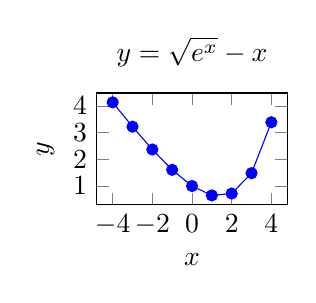
\begin{tikzpicture}
  \begin{axis}[width=4cm,height=3cm,
      title={$y=\sqrt{e^x}-x$},
      xlabel=$x$,ylabel=$y$]
    \addplot[blue,mark=*]
      expression[domain=-4:4,samples=9]
      {sqrt(exp(x))-x};
  \end{axis}
\end{tikzpicture}
%% *** END OF EXAMPLE CODE ***

\end{document}
